\chapter{Analysis}
\label{chap:analysis}
    \section{Hardware}
        Opening the device we exposed the PCB, which is shown in Figure~\ref{fig:PCB}. 
        
        \begin{figure}[H]
            \centering
            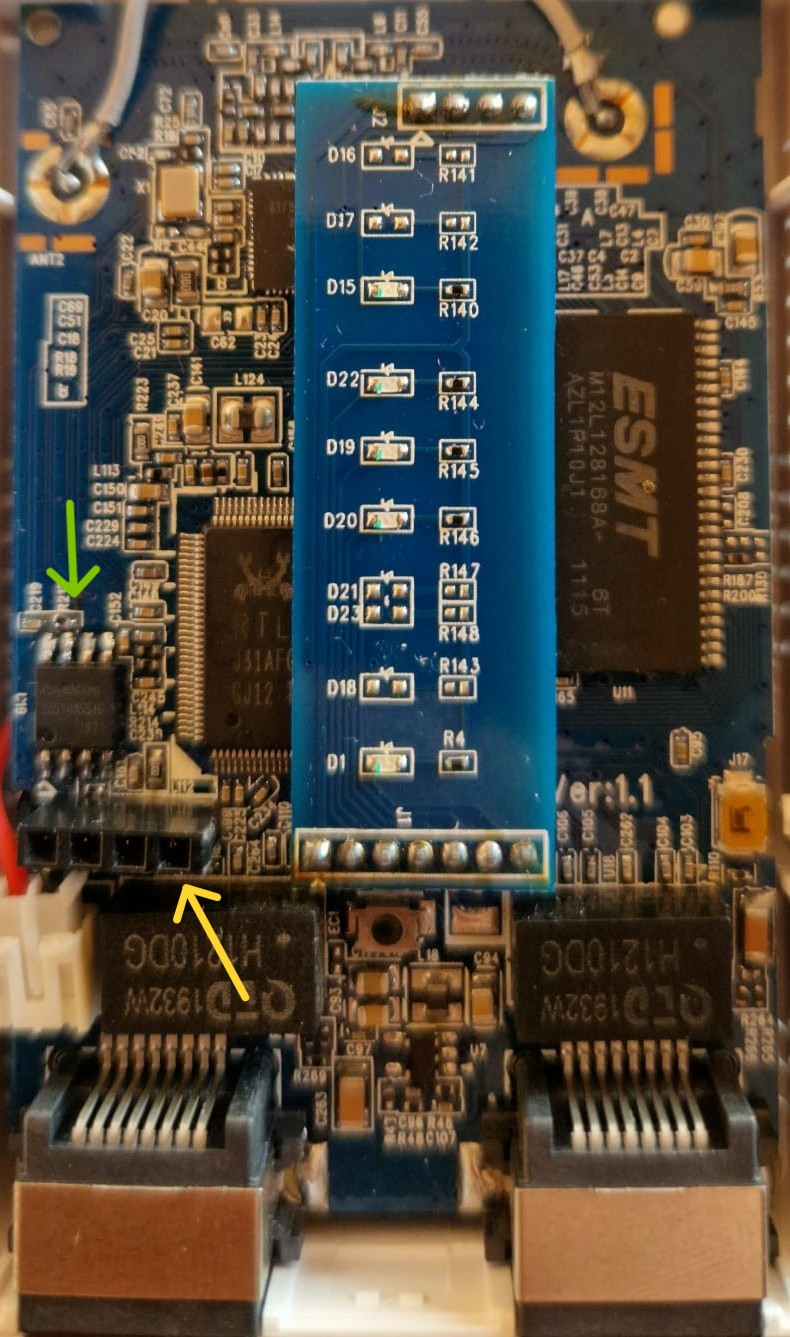
\includegraphics[width=0.5\textwidth]{../imgs/2.1-PCB.jpeg}
            \caption{PCB of the Aigital Wi-Fi Extender (after de-soldering the eeprom and inserting a connector to make the UART easier to read)}
            \label{fig:PCB}
        \end{figure}
        
        % We can see that the device is powered by a Mediatek MT7628NN\cite{MT7628NN}, which is a SoC designed for IoT devices.
        By a visual inspection of the PCB, we identified the pins of the UART interface, yellow arrow, the eeprom, green arrow and the following chips:
        \begin{itemize}
            \item ESMT M12L128168A, a 128 Mbit Synchronous DRAM (SDRAM) manufactured by ESMT (Elite Semiconductor Memory Technology Inc.). It is organized as 4 banks × 2,097,152 words × 16 bits, totalling 134,217,728 bits, and is designed for high-bandwidth, high-performance memory subsystems \cite{M12L128168A};
            \item RTL8196E, a compact SoC for low-power, low-cost networking applications. It combines a 400 MHz embedded CPU, a 5-port Fast Ethernet switch, and various peripherals (PCIe, SPI boot flash, DRAM interfaces, UART, and GPIO, among others) \cite{RTL8196E};
            \item RTL819ER, a highly integrated Wi-Fi module that can be easily integrated (given its self-contained design) and is optimized for low-power, high-speed operation. It has the ability to switch both analog and digital signals an to work with weak signals, making it ideal for a variety of applications, from IoT to game consoles \cite{RTL819ER}.
        \end{itemize}

        \subsection{UART}
            Using a digital multimeter, we individuated the pins of the UART interface (Figure~\ref{fig:uart}), which are (from left to right):
            \begin{itemize}
                \item Pin 1: VCC (red arrow)
                \item Pin 2: TX (yellow arrow)
                \item Pin 3: RX (green arrow)
                \item Pin 4: GND (blue arrow)
            \end{itemize}
            \begin{figure}[H]
                \centering
                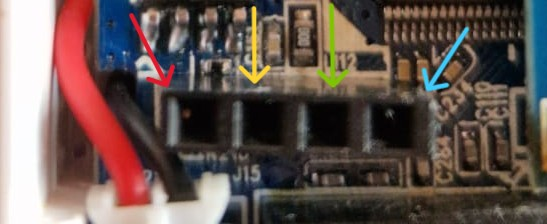
\includegraphics[width=0.8\textwidth]{../imgs/2.2-uart.jpeg}
                \caption{UART interface}
                \label{fig:uart}
            \end{figure}
            Once we identified the pins of the UART interface, we found, with some patience, the correct baud rate for the communication, which is 38400 baud.
            \\
            Booting the device and connecting to the UART interface with a USB-to-TTL adapter, we were able to read the boot log of the device, which is shown in Figure~\ref{fig:boot_log}.
            \begin{figure}[H]
                \centering
                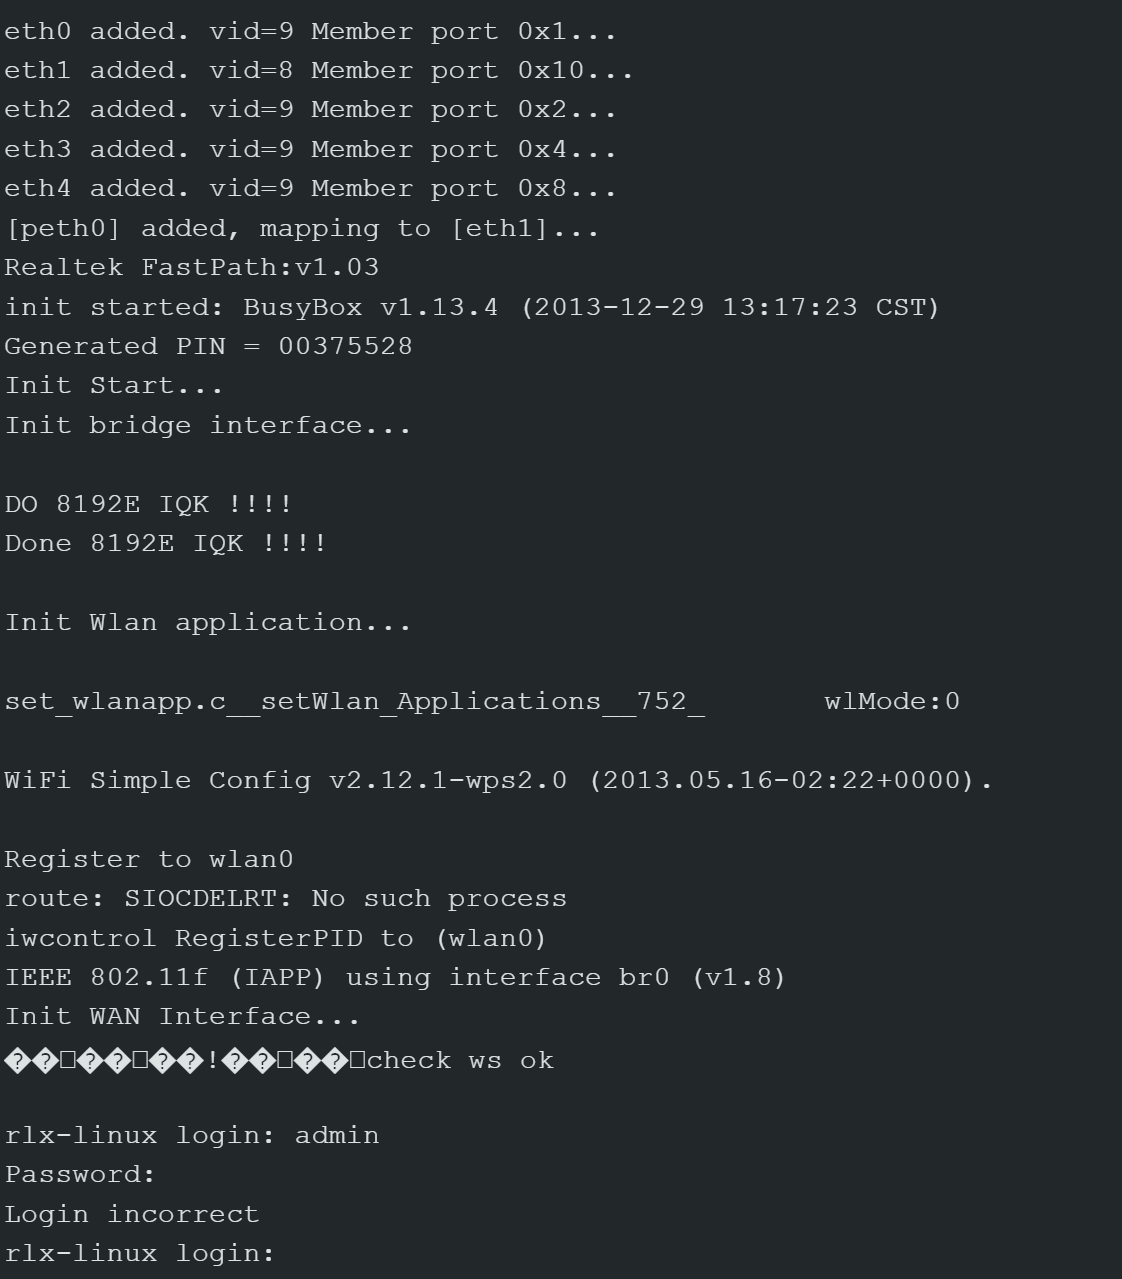
\includegraphics[width=0.8\textwidth]{../imgs/2.3-boot_log.png}
                \caption{Boot log of the device}
                \label{fig:boot_log}
            \end{figure}
            Unfortunately, no U-Boot console is available, but the boot log is still very useful for us, since it allows us to identify rlx-linux as the operating system running on the device. 
            The os we found, rlx-linux, is a custom open source Linux distribution for embedded devices.
            \\
            We tried to submit in the login  some common default credentials, but we were not able to log in to the device. 
            
            \subsection{Eeprom}
            
            The EEPROM is a BoyaMicro 25D16ASSIG (Figures~\ref{fig:eeprom}, ~\ref{fig:pin}, ~\ref{fig:logicDiagram}), which is a 16 Mbit (2 MB) SOP8 208mil SPI EEPROM.
            
            \begin{figure}[H]
                \centering
                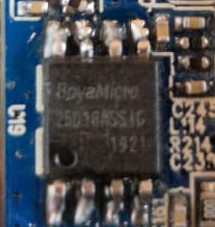
\includegraphics[width=0.5\textwidth]{../imgs/2.4-eeprom.jpeg}
                \caption{EEPROM}
                \label{fig:eeprom}
            \end{figure}
            \begin{figure}[H]
                \centering
                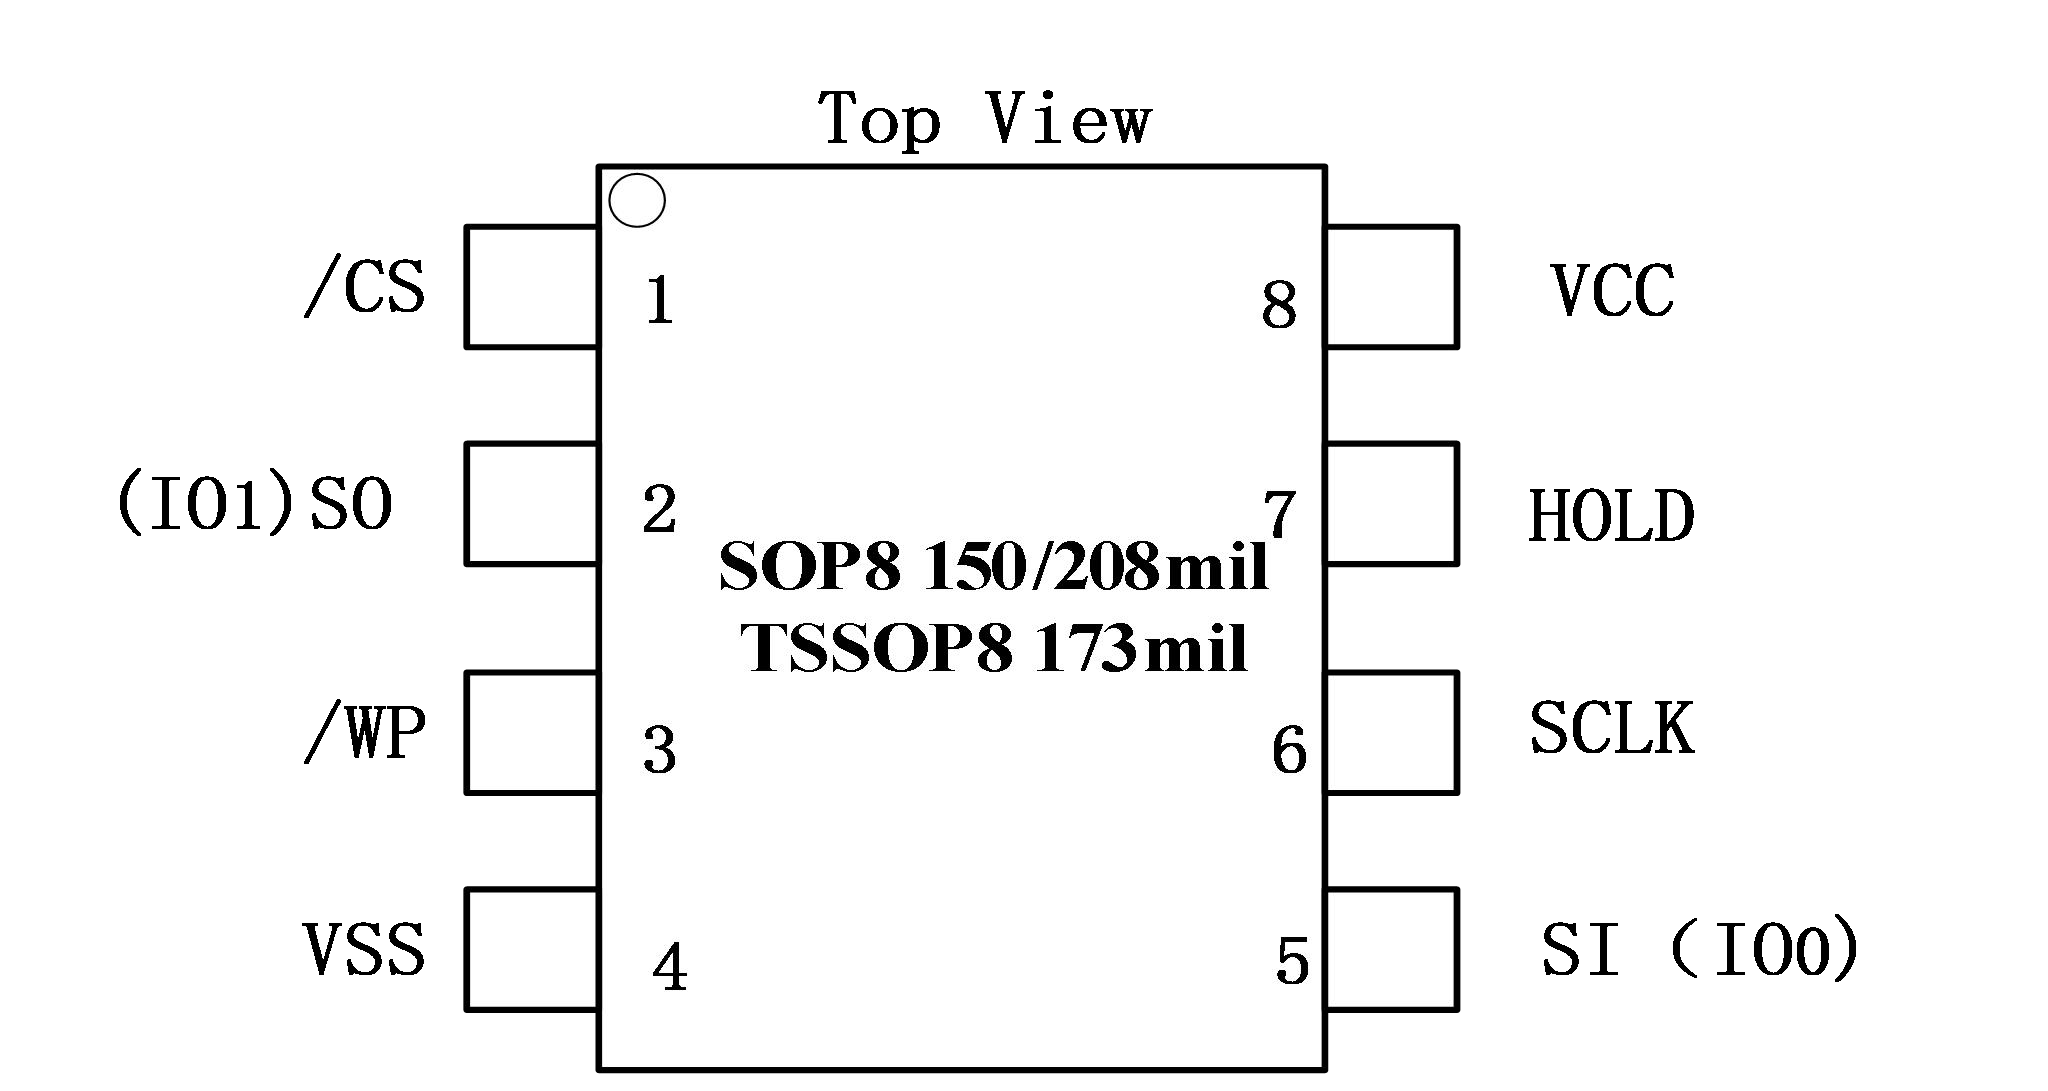
\includegraphics[width=0.5\textwidth]{../imgs/BY25D16AS/2.png}
                \caption{EEPROM Pin Configuration\cite{boya-micro}}
                \label{fig:pin}
            \end{figure}
            \begin{figure}[H]
                \centering
                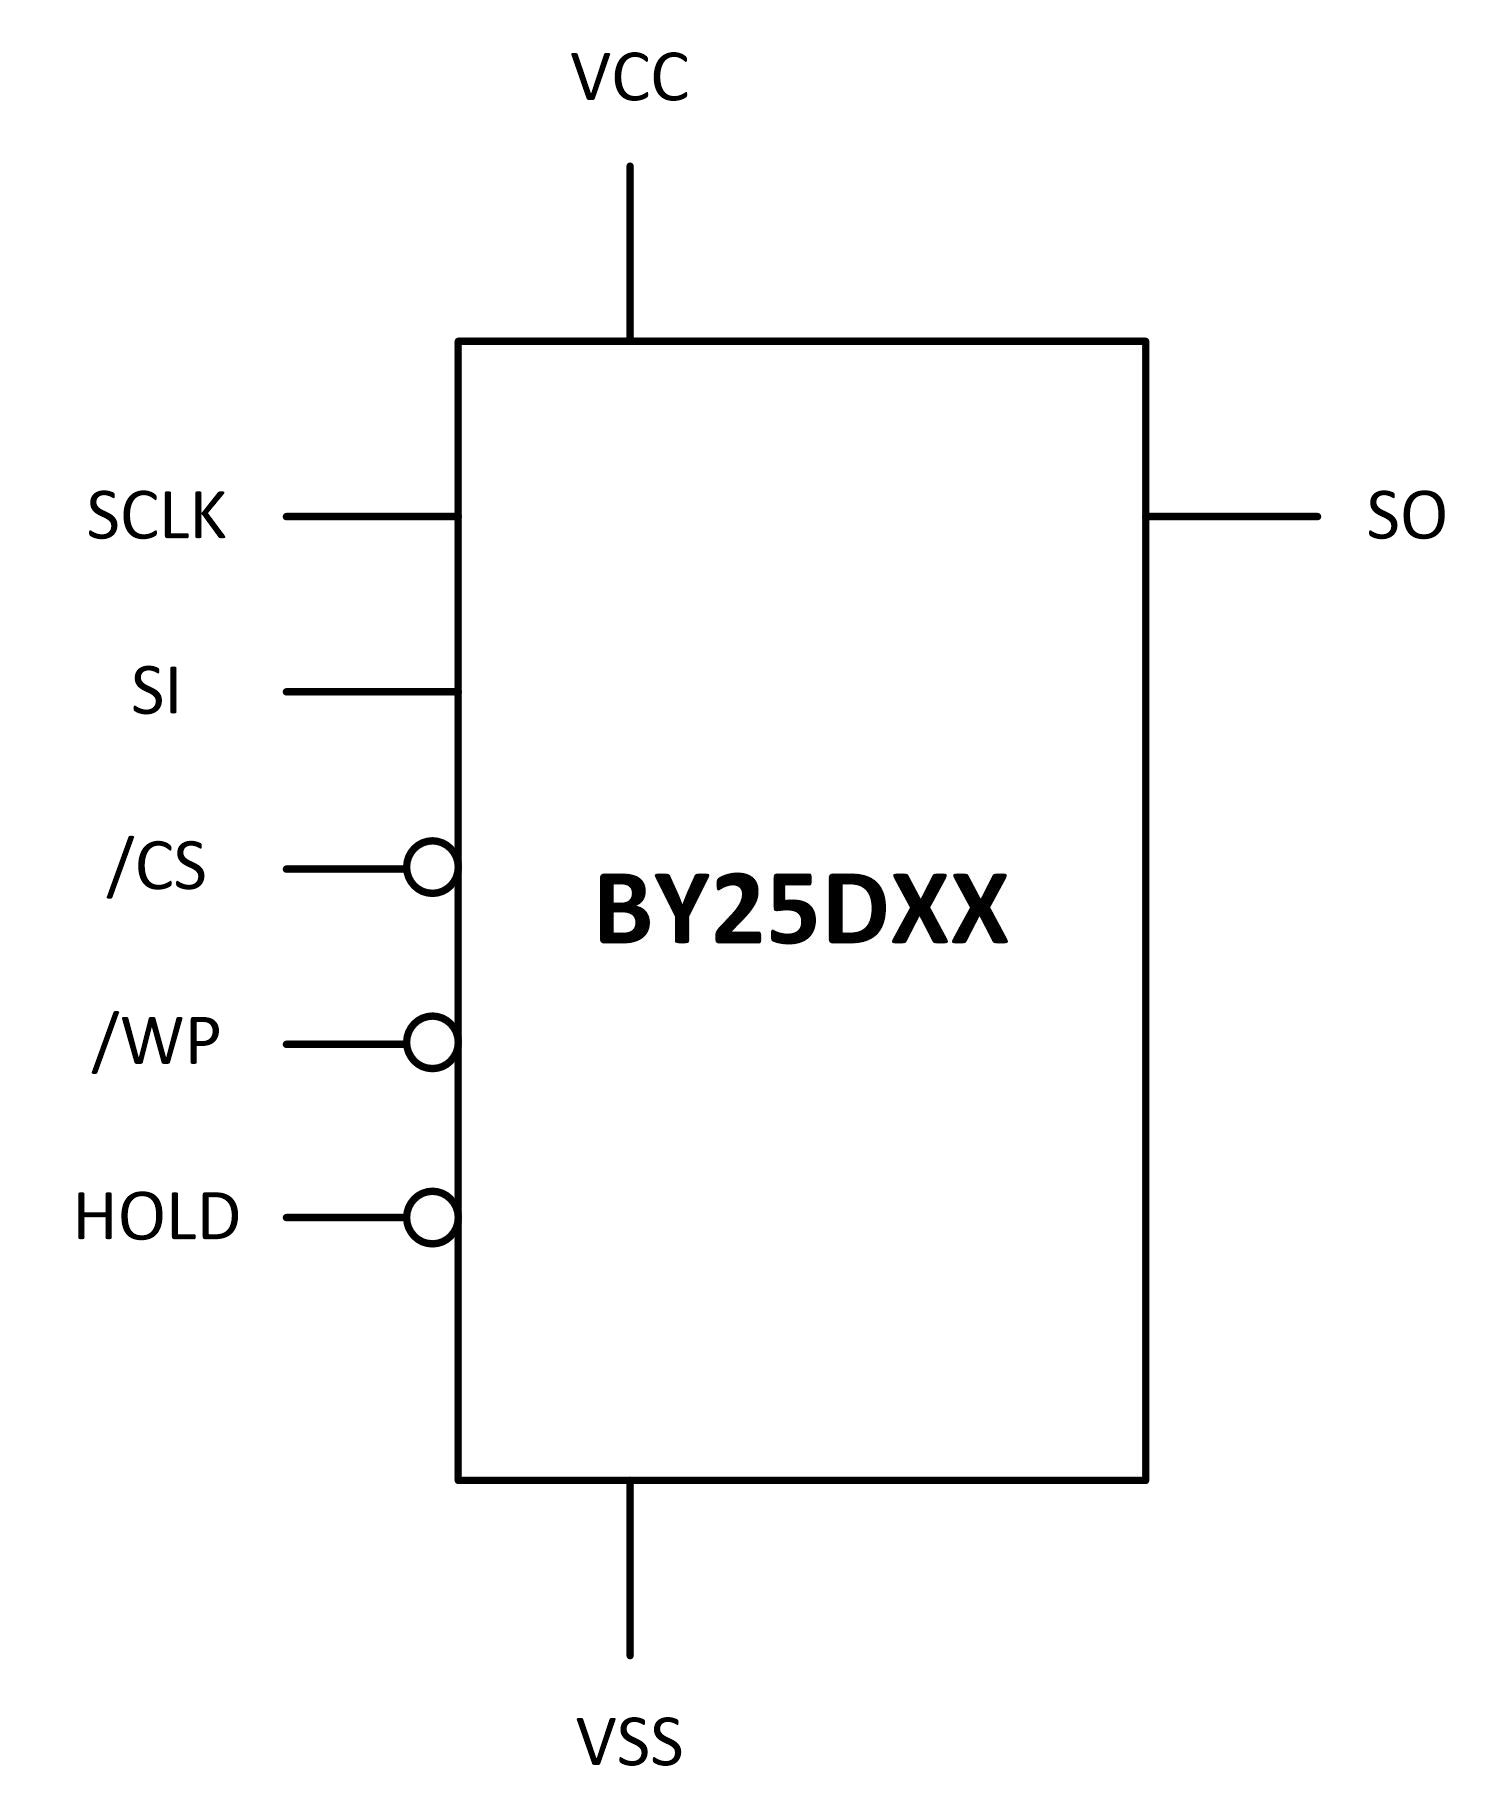
\includegraphics[width=0.5\textwidth]{../imgs/BY25D16AS/1.png}
                \caption{EEPROM Logic Diagram\cite{boya-micro}}
                \label{fig:logicDiagram}
            \end{figure}
            
    \section{Information Gathering}
        There isn't much information available about the device's manufacturer. The information that can be found online is mostly available on the Wayback Machine \cite{aigital.com}. From this information, it is clear that Aigital is a brand operated by a Chinese company based in Shenzhen: Shenzhen Zhuqiao Shuma Technology Co., Ltd \cite{registrazione}, whose products mainly include Bluetooth devices, antennas, and Wi-Fi devices \cite{aigital.com/gywm}.
        \\
        Although the device bears the FCC mark, we were unable to find any useful information about it on official websites such as \url{https://apps.fcc.gov/oetcf/eas/reports/GenericSearch.cfm} or unofficial ones such as \url{https://fccid.io} 
        \\
        While searching for information online, we immediately find several important results, one of which is Matteo Mandolini’s security analysis \cite{mandomat}, which identifies some very serious security vulnerabilities that have been assigned the CVEs mentioned earlier.
        \\ 
        However, we need to delve deeper into the information in the analysis in order to achieve our project objectives.
        \\
        
    \section{Software}
        To analyze how the router works, you need to obtain its firmware. However, as mentioned in the previous sections, the device does not provide any interface during the boot phase, making it necessary to dump the EEPROM memory.
        
        \subsection{Eeprom Dumping}
            To dump the EEPROM memory, we used a CH341A programmer with an SOIC clip. Initially, we attempted to dump the memory directly from the PCB. However, we noticed that when the programmer powered the EEPROM, it also powered the rest of the board, which caused excessive current draw and interference. We were therefore forced to desolder it in order to retrieve its contents.
            \begin{figure}[H]
                \centering
                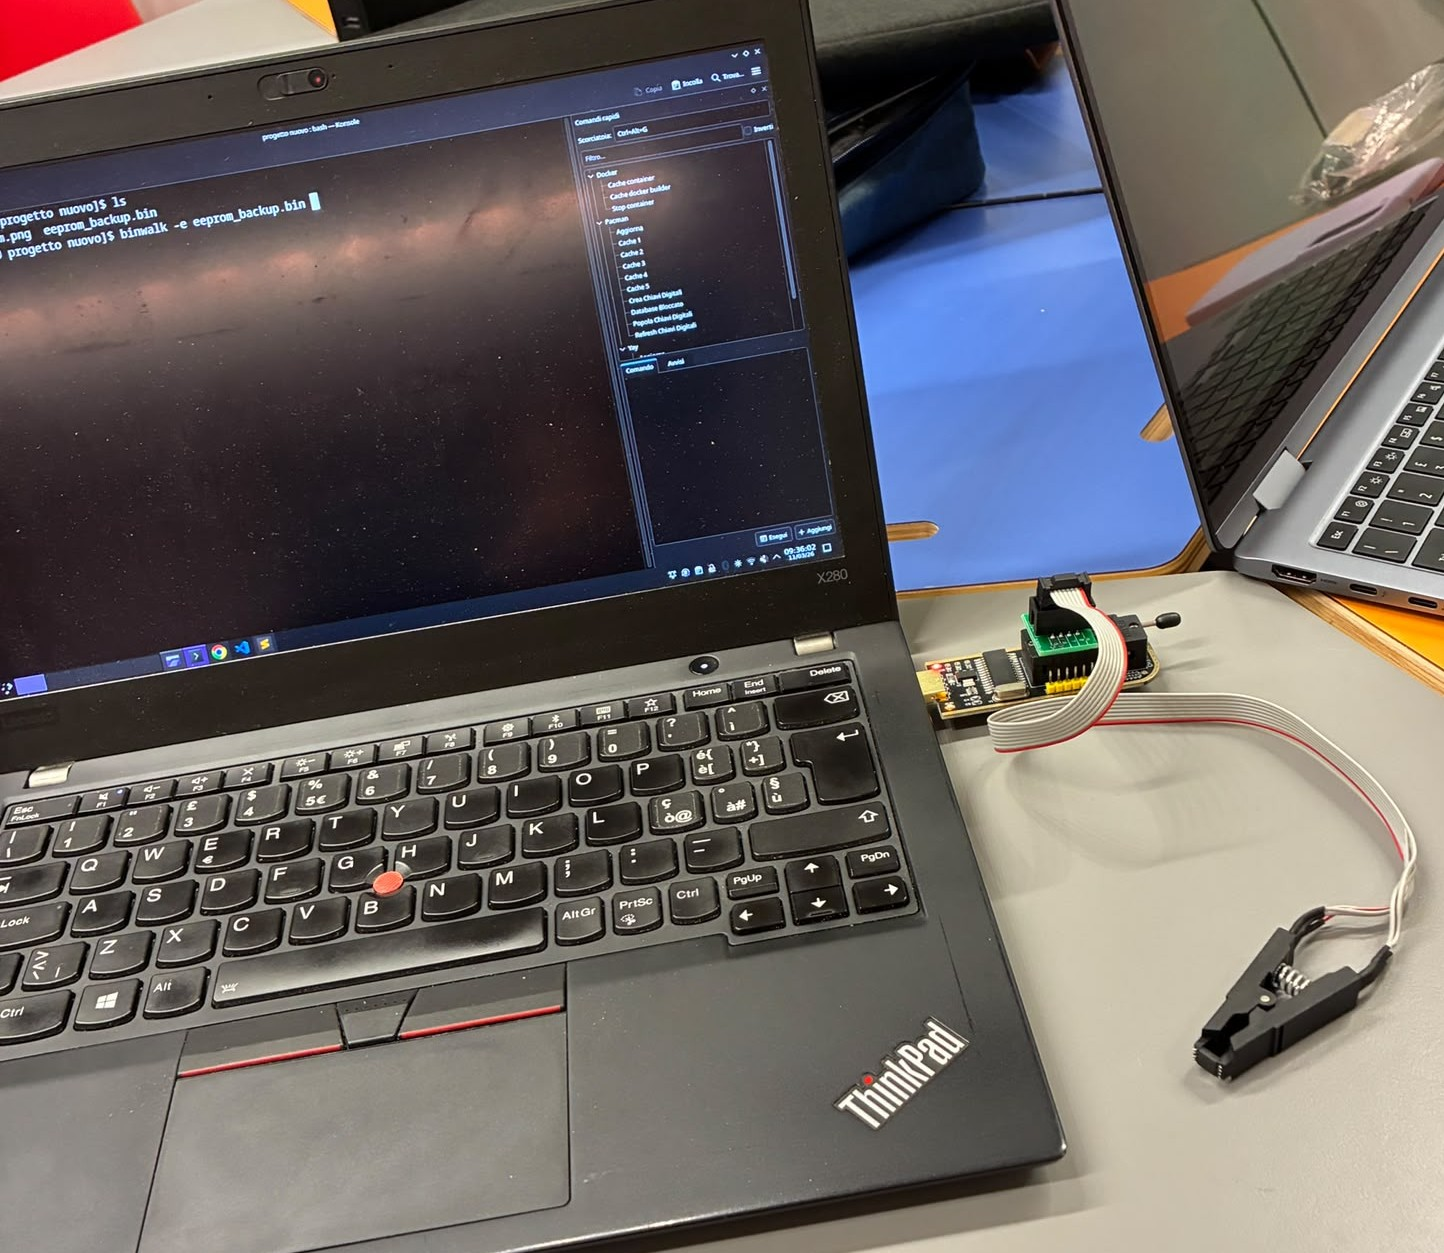
\includegraphics[width=0.9\textwidth]{../imgs/2.5-dumping_eeprom.jpeg}
                \caption{Dumping the EEPROM memory using SOIC clip}
                \label{fig:dumping_eeprom}
            \end{figure}
            As you can see in Figure~\ref{fig:dumping_eeprom}, we were forced to use the SOIC clip even after desoldering the EEPROM, since the EEPROM was too large for the socket we had.
            
            \begin{figure}[H]
                \centering
                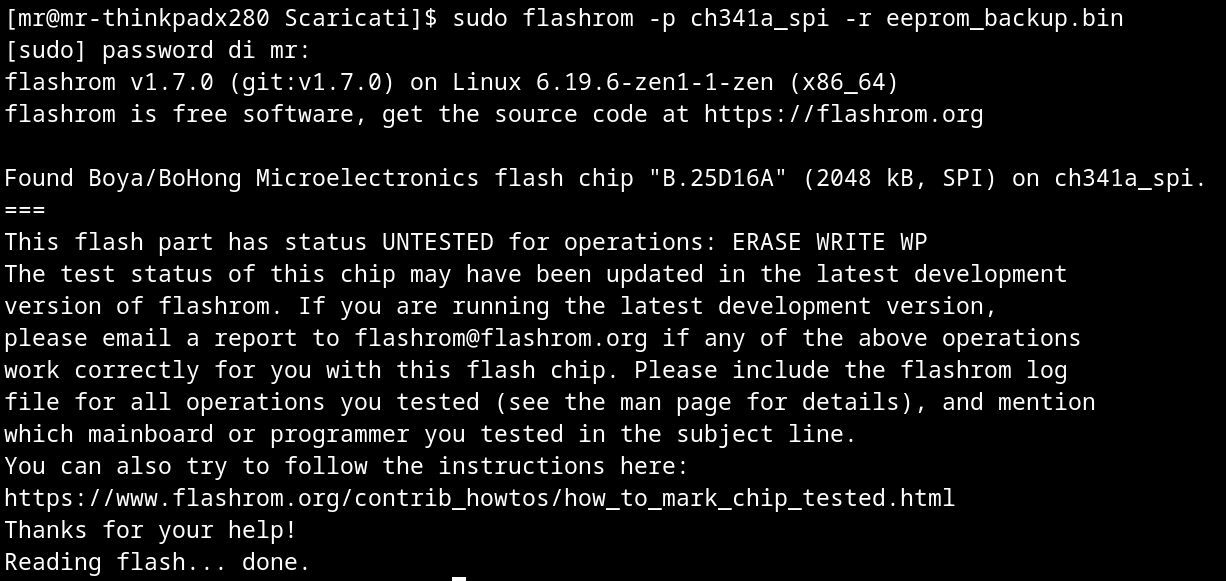
\includegraphics[width=0.9\textwidth]{../imgs/2.6-dump_iniziale_eeprom.png}
                \caption{EEPROM memory dump with flashrom command}
                \label{fig:dump}
            \end{figure}
            The dump (Figure~\ref{fig:dump}) was performed using the following command:
\begin{lstlisting}[language=bash]
sudo flashrom -p ch341a_spi -r eeprom_backup.bin
\end{lstlisting}
            Specifically:
        \begin{itemize}
            \item flashrom is a utility for reading, writing, erasing (and more) memory chips. It supports a wide range of protocols, including SPI, which is used by our \cite{flashrom} memory;
            \item -p is the option that specifies the programmer used for operations on the \cite{flashrom} memory chip; in our case, CH341A\_spi;
            \item -r is the option that specifies the destination file for the \cite{flashrom} memory read operation; in our case, eeprom\_backup.bin.
        \end{itemize}

        Then we analized with binwalk (Figure~\ref{fig:binwalk}) the binary that we extracted from EEPROM.
        \\
        Specifically, the binwalk analysis reveals that the firmware is divided into four blocks:
        \begin{itemize}
            \item 0x1310: small LZMA blob (approximately 17 KB compressed and 55 KB decompressed). Located immediately after the firmware header;
            \item 0x10010: 121 KB BZIP2 blob;
            \item 0x32818: 879 KB of compressed data that expands to approximately 3 MB of data, typical behavior for a compressed Linux kernel;
            \item 0x10A000: root filesystem of our device. Despite its size (128 KB), it appears to be complete.
        \end{itemize}        

        \begin{figure}[H]
            \centering
            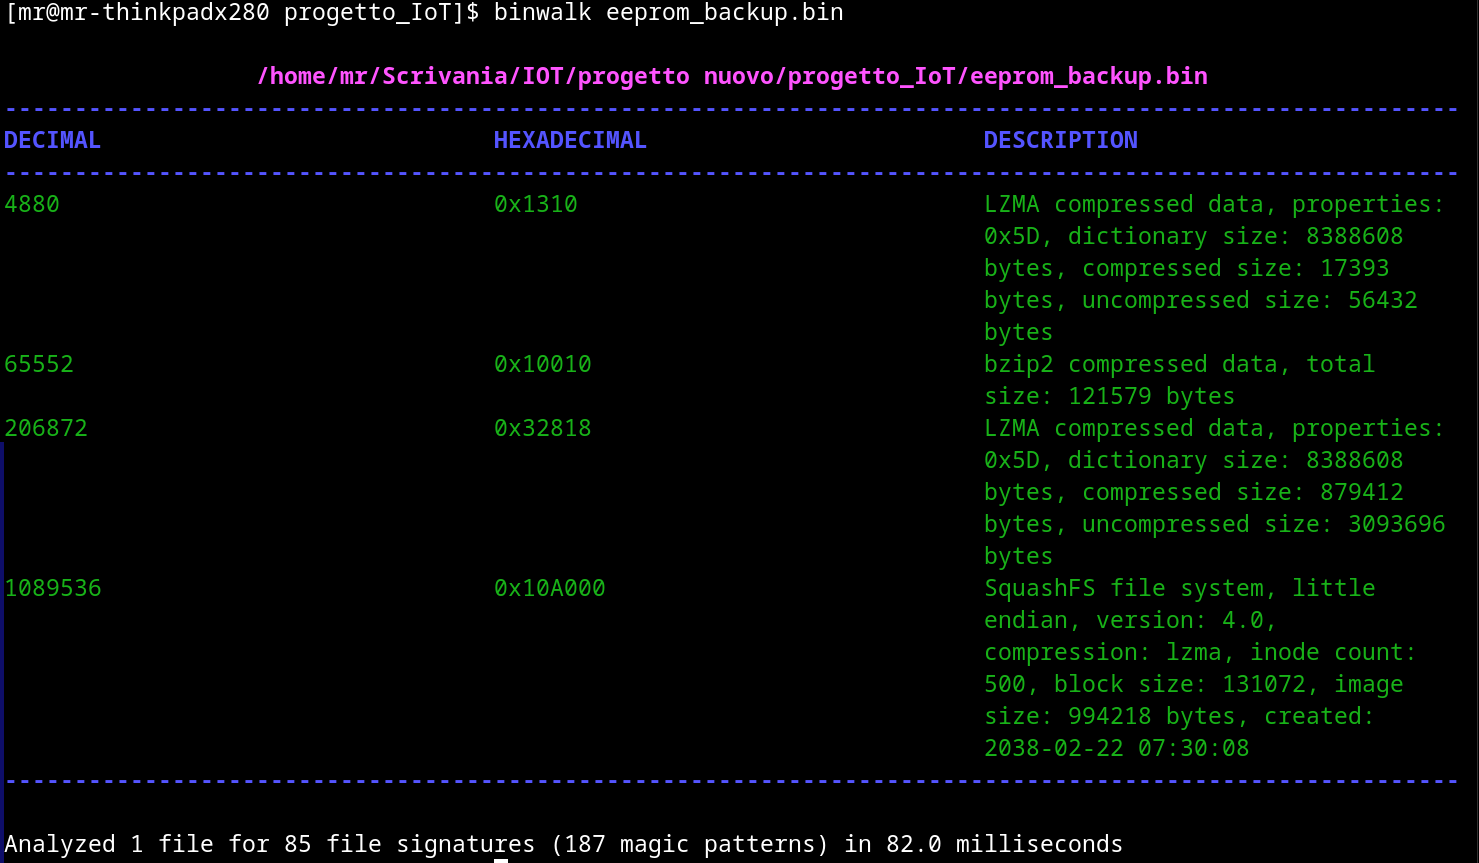
\includegraphics[width=0.9\textwidth]{../imgs/2.7-binwalk.png}
            \caption{Firmware extraction}
            \label{fig:binwalk}
        \end{figure}

        We then extracted everything using the -e option of binwalk, so that we could proceed with the analysis of the binaries contained within it.
        
        \subsection{Binary Analysis}

              After extracting the firmware, we started by inspecting the content of the recovered filesystem and the binaries involved in the web management interface. The most relevant executable for our analysis was
              the Boa web server, located at \emph{/bin/boa}.
              \\
              Boa is responsible for serving the administrative web interface and for dispatching the requests sent to the \emph{/boafrm/} endpoints. During the emulation phase, the HTTP headers confirmed that the
              server version used by the device is \emph{Boa/0.94.14rc21} \cite{mandomat}.
              \\
              BOA is a web server, ideal for use in embedded environments, created in 1995 and maintained until 2005. 
              Although it has not been maintained for more than two decades, it is still in use today.
              BOA suffers from a number of rather serious security vulnerabilities:
              \begin{itemize}
                  \item CVE-2017-9833: This vulnerability allows attackers to access arbitrary files on the server. It exploits the injection of "../.." using the FILECAMERA variable, enabling unauthorized file reading with root privileges.
                  \item CVE-2022-44117: This vulnerability allows SQL injection via the username parameter. However, it is disputed by some sources since Boa does not ship with SQL support.
              \end{itemize}
              However, since these vulnerabilities are not part of the project's original concept, we did not consider it necessary to investigate them further.
              \\
              The configuration file used by Boa was also found inside the root filesystem at \emph{/etc/boa/boa.conf}. The presence of this file was important because it allowed us to understand how the web server
              maps URLs to files and handlers. The static web pages were served from the web directory used by the firmware, while the dynamic operations were handled through specific endpoints under \emph{/boafrm/}.
              \\
              To identify the functions involved in the vulnerabilities, we analyzed the Boa binary with Ghidra. In particular, we focused on the handlers related to authentication and command execution. The endpoint \emph{/boafrm/formSysCmd} was especially relevant for the later RCE analysis, as its role was identified thanks to the information provided by the corresponding CVE documentation. \cite{mandomat}
              \\
              The corresponding client-side page was also present in the extracted web resources as \emph{webcmd.htm}. This page contains a form that submits a parameter called \emph{sysCmd} to the Boa handler:

\begin{lstlisting}[language=xml]
<form action=/boafrm/formSysCmd method=POST name="formSysCmd">
    <input type="text" name="sysCmd">
</form>
\end{lstlisting}

              This finding was relevant because it showed that command execution was an intended management feature in the original firmware. Whether access to this feature was correctly restricted is discussed in \cite{mandomat}.
              \\
              We also inspected the web pages used by the administrative interface. The login page was identified as \emph{login.htm}, and the login form submitted credentials to \emph{/boafrm/formLoginHtm}. The structure of the login request later allowed us to automate authentication during testing. The relevant fields are \emph{username}, \emph{password}, \emph{submit-value}, and \emph{lang\_select}.
              \\
              Another relevant part of the binary analysis concerned the relationship between Boa and the Realtek configuration libraries. Several web pages and Boa handlers depend on Realtek-specific NVRAM/MIB
              functions. These functions are provided by libraries such as \emph{/lib/libapmib.so}. During the analysis, this dependency became important because many crashes observed in Firmadyne were caused not by
              Boa itself, but by incomplete emulation of this configuration layer.
              \\
              The Boa binary was therefore analyzed in two ways:
              \begin{itemize}
                  \item statically, with Ghidra, to identify relevant handlers and code paths;
                  \item dynamically, during Firmadyne execution, to observe which requests triggered sockets, handlers, crashes, or command execution.
              \end{itemize}

              The screenshots below (Figure~\ref{fig:boaGhidra}) shows the function of the Boa binary opened in Ghidra, highlighting the specific function responsible for triggering the RCE vulnerability, which will be analyzed in detail in Chapter 4.


          \begin{figure}[H]
                \centering
                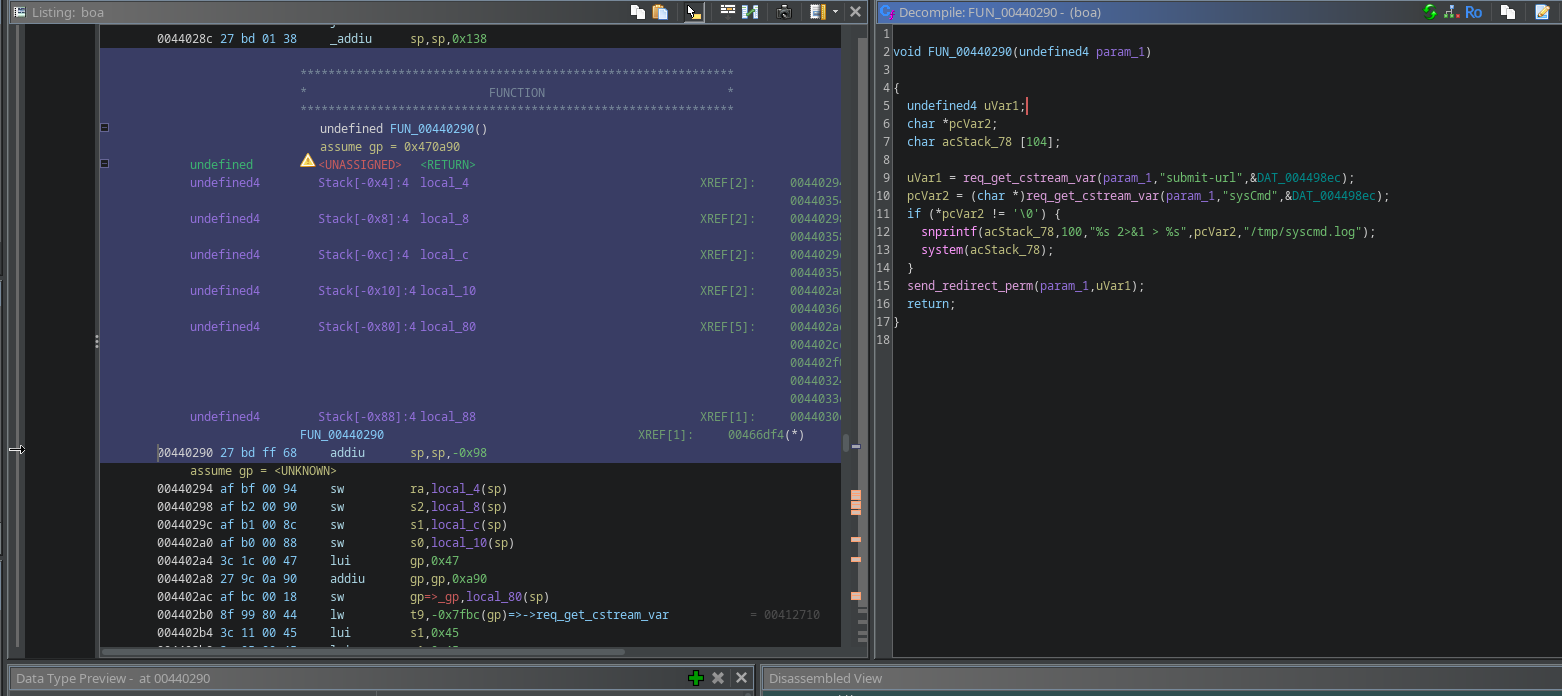
\includegraphics[width=0.9\textwidth]{../imgs/2.8-Boa_ghidra.png}
                \caption{Boa binary analyzed with Ghidra}
                \label{fig:boaGhidra}
            \end{figure}

              At this stage of the project, the binary analysis gave us three essential pieces of information:
              \begin{itemize}
                  \item the web server used by the device is Boa;
                  \item the authentication and command execution logic is implemented through Boa handlers;
                  \item the web interface depends heavily on Realtek-specific configuration functions.
              \end{itemize}

              These observations guided both the exploitation phase and the later patching phase.

          \subsection{Firmware Emulation}
              \label{sec:firmware emulation}

              After the hardware problems described in the introduction, we continued the analysis by emulating the firmware. The goal was not only to boot the extracted filesystem, but also to obtain a working
              environment where the web server and the relevant vulnerabilities could be tested.
              \\
              We used Firmadyne to emulate the firmware in a QEMU-based MIPS environment. Since the device is based on a Realtek platform, we used the MIPS big-endian configuration.
              \\
              The extracted root filesystem was packed into a Firmadyne-compatible archive:

\begin{lstlisting}[language=bash]
tar --numeric-owner -czf firmadyne/images/1.tar.gz \
    -C tentativo_dimensione/squashfs-root .
\end{lstlisting}

              The emulated disk image was then created with:

\begin{lstlisting}[language=bash]
cd firmadyne
sudo ./scripts/makeImage.sh 1 mipseb
\end{lstlisting}

              Finally, the firmware was started interactively with \emph{./scripts/run.mipseb.interactive.sh 1}.
              \\
              In order to make the firmware usable during emulation, we modified the startup configuration. The root account in \emph{/etc/passwd} was configured with an empty password field:

\begin{lstlisting}[language=bash]
root::0:0:root:/:/bin/sh
\end{lstlisting}

              Moreover, \emph{/etc/inittab} was modified so that the system spawns a shell directly:

\begin{lstlisting}[language=bash]
::respawn:-/bin/sh
\end{lstlisting}

              These changes were introduced only to simplify the emulation workflow. They allowed us to access the emulated firmware shell directly and configure the environment required for the tests.
              \\
              Once the firmware was running, the network had to be configured manually. We assigned the emulated firmware the same IP address used by the original web interface. The configuration was performed inside
              Firmadyne with the following commands:

\begin{lstlisting}[language=bash]
mkdir -p /proc
mount -t proc proc /proc
ifconfig eth0 192.168.10.253 netmask 255.255.255.0 up
route add default gw 192.168.10.100
\end{lstlisting}

               On the host side, the TAP interface used by QEMU/Firmadyne was configured manually. We brought the interface up, removed any previous address, and assigned the host address used throughout the tests:

\begin{lstlisting}[language=bash]
sudo ip link set qemu-tap0 up
sudo ip addr flush dev qemu-tap0
sudo ip addr add 192.168.10.100/24 dev qemu-tap0
\end{lstlisting}

                This placed the host machine and the emulated firmware in the same subnet. With this configuration, the emulated firmware could communicate with the host at \emph{192.168.10.100}. This was necessary
                for HTTP access to the web interface, ICMP testing, TFTP transfers, and reverse shell connections.

                For example, the \emph{nc} binary used during the RCE tests was transferred with:

\begin{lstlisting}[language=bash]
cd /tmp
tftp -g -l /tmp/nc -r nc 192.168.10.100
chmod +x /tmp/nc
\end{lstlisting}

              A major objective of the emulation was to run the original Boa web server. After the initial boot, we verified that Boa was running with \emph{ps | grep boa}. From the host machine, the web server was
              reachable at \emph{http://192.168.10.253/}. We checked the HTTP server with \emph{curl -I http://192.168.10.253/}, and the response confirmed that the emulated firmware was serving the web interface
              through \emph{Boa/0.94.14rc21}.

              During this phase, we discovered that simply running the original web application was not enough. Several pages caused segmentation faults because they relied on Realtek-specific NVRAM/MIB values that
              Firmadyne did not emulate correctly. The errors were typically related to calls performed through \emph{libapmib.so} or through internal Boa handlers that expected valid configuration data from the
              device.

              For this reason, before using the emulated firmware for the exploitation tests, we created a stabilized version of the original Boa binary. This version was not meant to fix the vulnerabilities under
                analysis, but only to make the original web server usable inside Firmadyne.

                During the first emulation attempts, Boa crashed when some authenticated pages triggered Realtek-specific MIB/NVRAM access paths. These crashes were caused by missing or incomplete configuration
                structures in the emulated environment, not by the CVEs themselves. The serial output showed repeated segmentation faults after requests to web pages that queried configuration values through the Realtek
                libraries.

                To avoid confusing emulation failures with security behavior, we patched only the Boa code paths responsible for those Firmadyne-specific crashes. The vulnerable command execution handler was
                intentionally left unchanged in this stabilized version. In this way, the resulting binary still behaved as the original vulnerable server for the RCE test, while being stable enough to keep the web
                interface reachable.

                The stabilization patches were applied to the original Boa binary at the following file offsets:

\begin{lstlisting}[language=bash]
0x27de4
0x30bb0
0x30be0
\end{lstlisting}

  Since the executable is loaded at virtual address \emph{0x00400000}, the corresponding addresses visible in Ghidra are:

\begin{lstlisting}[language=bash]
0x00427de4
0x00430bb0
0x00430be0
\end{lstlisting}

  At these addresses, the original instructions belonged to code paths that expected valid pointers returned by Realtek-specific configuration routines. In Firmadyne, those pointers could be null or otherwise invalid,
  causing Boa to crash during page rendering. The stabilization patches replaced the unsafe dereference paths with MIPS \emph{nop} instructions or, where required by the local control flow, with an early return
  sequence. This kept the binary layout unchanged and avoided modifying the security-relevant RCE handler at \emph{0x00440290}.

  These changes should therefore be considered emulation-stability patches, not security patches. The binary obtained after these changes was saved as \emph{boa.before-boaPatched}: it is the pre-security-patch Boa used
  to reproduce the RCE, but already stabilized for the emulated environment.

  Starting from this stabilized vulnerable binary, we later produced \emph{boa.patched-stable}, which keeps the same Firmadyne stability patches and additionally disables the RCE handler. The RCE-specific binary patch
  is discussed separately in Chapter~\ref{chap:fixing}.

              In parallel, we also stabilized the web resources. The approach was conservative:
              \begin{itemize}
                  \item keep the real Boa binary running inside the firmware;
                  \item keep the original login flow;
                  \item preserve the look and structure of the web interface;
                  \item avoid unstable dynamic handlers not required for the demonstration;
                  \item create stable versions of the pages needed during the tests.
              \end{itemize}

              The stabilized pages included \emph{home.htm}, \emph{status.htm}, \emph{wzd\_ap.htm}, \emph{wlbasic.htm}, \emph{tcpiplan.htm}, and \emph{admin.htm}. They were designed to reproduce the relevant
              structure of the original interface, including the main sections \emph{Home}, \emph{Wizard}, \emph{Wireless}, \emph{TCP/IP}, and \emph{Management}, together with the configuration panels
              \emph{Wireless}, \emph{LAN}, \emph{WAN}, and \emph{System}.

              This produced an emulated web interface that was stable enough for the rest of the project. So this was not a perfect full emulation of all proprietary Realtek configuration
              logic. However, it was sufficient for the security analysis because:
              \begin{itemize}
                  \item the firmware was running in Firmadyne;
                  \item the Boa web server was the real server used by the device;
                  \item the login and navigation were functional;
                  \item the vulnerable and patched behaviors could be tested in a controlled way.
              \end{itemize}

          \subsection{Firmware Analysis}

              After obtaining a stable emulation environment, we analyzed the firmware from the point of view of the components involved in the vulnerabilities. The analysis focused on the interaction between the web
              interface, the Boa server, and the underlying system commands.

              The first relevant observation was that the web interface is not a simple collection of static pages. It is composed of:
              \begin{itemize}
                  \item static HTML, CSS and JavaScript files;
                  \item Boa handlers exposed through \emph{/boafrm/};
                  \item Realtek-specific configuration functions used to read and write device settings;
                  \item system utilities invoked by the web server.
              \end{itemize}

              The login mechanism is implemented through a POST request to \emph{/boafrm/formLoginHtm}. The request contains the username, password and language selector. During the emulated tests we used the
              credentials \emph{admin/admin}. The same login flow was later reused by the exploit script to automate access to the web interface before sending commands.

              The second relevant component was the command execution interface. The web resources include a page named \emph{webcmd.htm}, which submits commands to \emph{/boafrm/formSysCmd}. This handler is the key
              component for the RCE vulnerability. At the analysis stage, we did not yet patch or exploit it; we identified it as the relevant attack surface for Chapter 3.

              The third relevant component was the management of wireless configuration values, especially the SSID. The SSID is a user-controlled value that is displayed back in the web interface. This behavior is
              security-sensitive because, if the value is inserted into the DOM\footnote{The Document Object Model (DOM) is the browser's internal representation of a web page, and it exposes its elements as objects that can be read and modified by client-side scripts} without escaping, it can lead to cross-site scripting.

              The unsafe rendering pattern is represented by code that inserts a string using \emph{innerHTML}:

\begin{lstlisting}[language=bash]
target.innerHTML = ssid;
\end{lstlisting}

              A safer rendering pattern is to treat the value as text:

\begin{lstlisting}[language=bash]
target.textContent = ssid;
\end{lstlisting}


              The practical exploitation and mitigation of this issue are discussed later in Chapters 3 and 4. In this chapter, the important result is that the firmware exposes user-controlled configuration values
              through the web interface, and these values must be handled carefully.

              During the firmware analysis we also prepared two Boa versions for later testing:
              \begin{itemize}
                  \item a vulnerable version, used to reproduce the original behavior;
                  \item a patched stable version, used to verify that the web application remains usable while the RCE is blocked.
              \end{itemize}

              The two relevant binaries are \emph{boa.before-boaPatched} and \emph{boa.patched-stable}, as anticipated in the previous section. The active binary inside the root filesystem is always named \emph{/bin/boa}.

              To switch between the two versions, we copied the desired binary over \emph{/bin/boa} and rebuilt the Firmadyne image. For example, to use the vulnerable version:

\begin{lstlisting}[language=bash]
cp tentativo_dimensione/squashfs-root/bin/boa.before-boaPatched \
    tentativo_dimensione/squashfs-root/bin/boa
\end{lstlisting}

              To use the patched version:

\begin{lstlisting}[language=bash]
cp tentativo_dimensione/squashfs-root/bin/boa.patched-stable \
    tentativo_dimensione/squashfs-root/bin/boa
\end{lstlisting}

              This approach allowed us to compare the behavior of the same emulated firmware under two different Boa binaries.

              In summary, the firmware analysis identified the components that are essential for the rest of the report:
              \begin{itemize}
                  \item Boa as the central web server;
                  \item \emph{/boafrm/formLoginHtm} as the login endpoint;
                  \item \emph{/boafrm/formSysCmd} as the command execution endpoint;
                  \item the SSID rendering logic as the relevant XSS sink;
                  \item the dependency on Realtek-specific MIB/NVRAM functions as the main challenge for emulation.
              \end{itemize}          